\documentclass[a4paper,12pt]{article}
\pagestyle{plain}
\usepackage[T1]{fontenc}
\usepackage{txfonts}
\sloppy
\usepackage{graphicx}
\begin{document}

\title{Assignment - Module 3}
\date{\today}
\author{Chidambaram P G, Fathima K M, Mohan S Nayaka, Muhassin Babu M M\\ Pathang V S, Selvam G, Suraj K}
\maketitle
\noindent
1. Write a short note on separate compilation [Section 11.6 - Sebesta]\\
\emph{Answer}:

When the size of a program is large, two practical problems become evident. One is that the organization of a program as a single collection of subprograms and abstract type definitions is inadequate and the second problem is that recompilation. For large programs, the cost of recompilation is significant. So, there is an obvious need to find ways to avoid recompilation of the parts of a program that are not affected by a change. The obvious solution to both of these problems is to organize programs into collections of logically related code and data, each of which can be compiled without recompilation of the rest of the program. An \textbf{encapsulation} is such a collection.

Encapsulations are often placed in libraries and made available for reuse in programs other than those for which they were written. Techniques for providing encapsulations have been evolving for some time. In languages that allow nested subprograms, programs can be organized by nesting subprogram definitions inside the logically larger subprograms that use them. This can be done in Ada, Fortran 95, Python, and Ruby. Even in languages that allow nested subprograms, they are not used as a primary organizing encapsulation construct.

\textbf{Encapsulation in C}

C does not provide complete support for abstract data types, although both abstract data types and multiple-type encapsulations can be simulated. In C, a collection of related functions and data definitions can be placed in a file, which can be independently compiled, acts as a library, and has an implementation of its entities. The interface to such a file, including data, type, and function declarations, is placed in a separate file called a \textbf{header file}.

Type representations can be hidden by declaring them in the header file as pointers to struct types. Implementation file includes definitions of struct types. This approach has the same drawbacks as the use of pointers as abstract data types in Ada packages -- namely, the inherent problems of pointers and the potential confusion with assignment and comparisons of pointers. The header file, in source form, and the compiled version of the implementation file are furnished to clients. When such a library is used, the header file is included in the client code, using an \#include pre-processor specification, so that references to functions and data in the client code can be type checked. The \#include specification also documents the fact that the client program depends on the library implementation file. This approach effectively separates the specification and implementation of an encapsulation. Although these encapsulations work, they create some insecurity. First, the documentation of the dependence of the client program on the library (and its header file) is lost. Second, the author of the library could change the header file and the implementation file, but the client could attempt to use the new implementation file (not realizing it had changed) but with the old header file, which the user had copied into his or her client program. Thus, it is the user's responsibility to ensure that both the header and implementation files are up-to-date. This is often done with a make utility (a dependency management tool).\\
\\
\noindent
2. Example and explanation of a simple attribute grammar,\\ \textit{[Sec. 4.2, page 166, Programming Language Pragmatics (Scott)]}\\
\emph{Answer}:

A grammar that generates properly formed constant expressions over the basic arithmetic operators, but it says nothing about their meaning. To tie these expressions to mathematical concepts, we need additional notation. The most common is based on attributes. The intent is that for any symbol S, S.val will be the meaning, as an arithmetic value, of the token string derived from S. We assume that the Val of a const is provided to us by the scanner. We must then invent a set of rules for each production to specify how the Vals of different symbols are related. In simple grammar, every production has a single rule. We shall see more complicated grammars later in which productions can have several rules. The rules come in two forms. \textit{Copy rules}, they specify that one attribute should be a copy of another. The other rules invoke \textit{semantic functions} (sum, quotient, additive inverse, etc.). In general Semantic functions can be arbitrarily complex functions specified by the language designer. Each semantic function takes an arbitrary number of arguments (each of which must be an attribute of a symbol in the current production: no constants, global variables,
etc.), and each computes a single result, which must likewise be assigned into an attribute of a symbol in the current production. When more than one symbol of a production has the same name, subscripts are used to distinguish them. These subscripts are solely for the benefit of the semantic functions; they are not part of the context-free grammar itself.
In a strict definition of attribute grammars, copy rules and semantic function calls are the only two kinds of permissible rules. In practice, it is common to allow rules to consist of small fragments of code in some well-defined notation (e.g., the language in which a compiler is being written) so that simple semantic functions can be written out ``in-line.'' These code fragments are not allowed to refer to any variables or attributes outside the current production. In our examples we use a $\triangleright$    symbol to introduce each code fragment corresponding to a single semantic function.

Semantic functions must be written in some already-existing notation, because
attribute grammars do not really specify the meaning of a program; rather, they provide a way to associate a program with something else that presumably has meaning. Neither the notation for semantic functions nor the types of the attributes themselves (i.e., the domain of values passed to and returned from semantic functions) is intrinsic to the attribute grammar notion. In the preceding example, we have used an attribute grammar to associate numeric values with the symbols in our grammar, using semantic functions drawn from ordinary arithmetic. In the code generation phase of a compiler, we might associate fragments of target machine code with our symbols, using semantic functions written in some existing programming language. If we were interested in defining the meaning of a programming language in a machine-independent way, our attributes might be domain theory \textit{denotations} (these are the basis of \textit{denotational semantics}). If we were interested in proving theorems about the behavior of programs in our language, our attributes might be logical formulas (this is the basis of \textit{axiomatic semantics}).\\
Example: An LR (bottom-up) grammar for arithmetic expressions composed of constants, with precedence and associativity:\\
\begin{quote}
E $\longrightarrow$ E  + T\\
E $\longrightarrow$ E  - T\\
E $\longrightarrow$ T\\
T $\longrightarrow$ T  * F\\
T $\longrightarrow$ T  / F\\
T $\longrightarrow$  F\\
F $\longrightarrow$ - F\\
F $\longrightarrow$ (E)\\
F $\longrightarrow$ const\\
\end{quote}
A simple attribute grammar for constant expressions, using the standard arithmetic operations.\\
\begin{quote}
1. $E_1$ $\longrightarrow$ $E_2$ + T \\
\verb+       +$\triangleright$ $E_1$.val := sum($E_2$.val + T.val)\\
2. $E_1$ $\longrightarrow$ $E_2$ - T \\
\verb+       +$\triangleright$ $E_1$.val := sum($E_2$.val - T.val)\\
3. E $\longrightarrow$  T \\
\verb+       +$\triangleright$ E.val := T.val\\
4. $T_1$ $\longrightarrow$ $T_2$ * F \\
\verb+       +$\triangleright$ $T_1$.val := product($T_2$.val * F.val)\\
5. $T_1$ $\longrightarrow$ $T_2$ / F \\
\verb+       +$\triangleright$ $T_1$.val := quotient($T_2$.val / F.val)\\
6. T $\longrightarrow$  F \\
\verb+       +$\triangleright$ T.val := F.val\\
7. $F_1$ $\longrightarrow$ $-F_2$\\
\verb+       +$\triangleright$ $F_1$.val := additive\_inverse($F_2$.val)\\
8. F $\longrightarrow$  (E) \\
\verb+       +$\triangleright$ F.val := E.val\\
9. F $\longrightarrow$ const\\
\verb+       +$\triangleright$ F.val := const\\
\end{quote}

\noindent
3. Determine the output for C++ code using pass-by-reference and using
pass-by-value methods for parameter passing using the following code:\\
\begin{quote}
void mystery(int\& a, int\& b, int c)\\
\{\\
\verb|    |a=b+c;\\
\verb|    |b=0;\\
\verb|    |c=0;\\
\}\\
void print (void)\\
\{\\
\verb|    |int x = 0, y = 1, z = 2;\\
\verb|    |mystery(x, y, z);\\
\verb|    |cout \verb|<<| x \verb|<<| ''  ''   \verb|<<| y \verb|<<| ''  '' \verb|<<| z;\\
\verb|    |mystery(x, y, z);\\
\verb|    |cout \verb|<<| x \verb|<<| ''  '' \verb|<<| y \verb|<<| ''  '' \verb|<<| z \verb|<<| endl;\\
\}\\
\end{quote}
\emph{Answer}:

Passing by reference refers to a method of passing arguments whereby the value of an argument whereby the value of the argument in the \emph{calling} function can be modified in the \emph{called} function. In C++, by default, parameters are passed by value. When srguments are passed by value, copies of arguments are received by the called function and thus changes made in the called functions are not reflected in the calling function.

Hence, in the mystery() function, changes made to the parameters a and b are reflected in the main() function, while the the third argument c remains unchanged in the main() function. Therefore, the output from this program is:\\
3  0  2\\
2  0  2\\

\noindent
4. Write a program to determine the factorial of an integer input with and without recursion.\\
\emph{Answer}:

The following is a C function (using recursion) to calculate the factorial:\\
\begin{quote}
long int factorial (int num)\\
\{\\
\verb|    |if ((num == 0) || (num == 1))\\
\verb|    |\{\\
\verb|        |return 1;\\
\verb|    |\}\\
\verb|    |else\\
\verb|    |\{\\
\verb|        | return (num * factorial (num - 1));\\
\verb|    |\}\\
\}\\
\end{quote}
\emph{Algorithm}:\\
\begin{enumerate}
\item START
\item If the input \textit{num} is either zero or one, return one (STOP).
\item Return the product of \textit{num} and the result of calling this function with argument of \emph{(num-1)}
\item STOP
\end{enumerate}
The same result can be achieved using iteration instead of recursion as follows:\\
\begin{quote}
long int factorial (int num)\\
\{\\
\verb|    |long int result = 1;\\
\verb|    |int i;\\
\verb|    |for (i = 1; i \verb|<=| num; i++)\\
\verb|    |\{\\
\verb|    |\verb|    |result = result * i;\\
\verb|    |\}\\
\verb|    |return result;\\
\}\\
\end{quote}
\emph{Algorithm}:\\
\begin{enumerate}
\item START
\item Initialise variables \textit{result} (to one) and \textit{i} to zero.
\item If \emph{i} is greater than \emph{num}, go to step 5.
\item Set the value of \emph{result} to the product of \emph{result} and \emph{i}
\item Return the value of the variable \emph{result}.
\item STOP
\end{enumerate}
\noindent
5. Draw the dependency graph for semantic rules associated with the productions listed below.
\begin{center}
\begin{tabular}{|c|c|}
\hline
Production &  Semantic Rules\\
\hline
A $\longrightarrow$ BC & B.inh = A.inh\\
&C.inh=A.inh-B.inh+B.syn\\
&A.syn=A.inh*B.inh+B.syn-C.inh/C.syn\\
\hline
B $\longrightarrow$ X &X.inh=something\\
& B.syn=B.inh+X.syn\\
\hline
C $\longrightarrow$ Y & Y.inh=something\\
& C.syn=C.inh+Y.syn\\
\hline
\end{tabular}
\end{center}
\emph{Answer}:

The simplest counter example is the single production A $\rightarrow$ B with synthesized attribute A.syn, inherited attribute B.inh, and rules A.syn=B.inh and B.inh=A.syn+1. This means to evaluate A.syn at the parent node we need B.inh at the child and vice versa.\\
A parse tree decorated with attributes, is called an annotated parse tree.\\
The graph just drawn is called the dependency graph. In addition to being generally useful in recording the relations between attributes, it shows the evaluation order can be used. \\
Evaluating L-Attributed :
Thus what we need is to find an evaluation order respecting the arrows. This is called a topological sort. The rule is that the needed ordering can be found if and only if there are no (directed) cycles. The algorithm is simple.
\begin{enumerate}
\item Choose a node having no incoming edges
\item Delete the node and all outgoing edges.
\item Repeat
\end{enumerate}

The rules for calculating A.syn, B.inh, and C.inh are shown in the table. The attribute A.inh would have been set by the parent of A in the tree; the semantic rule generating A.inh would be given with the production at the parent.
\begin{figure}[!bhp]
\centering
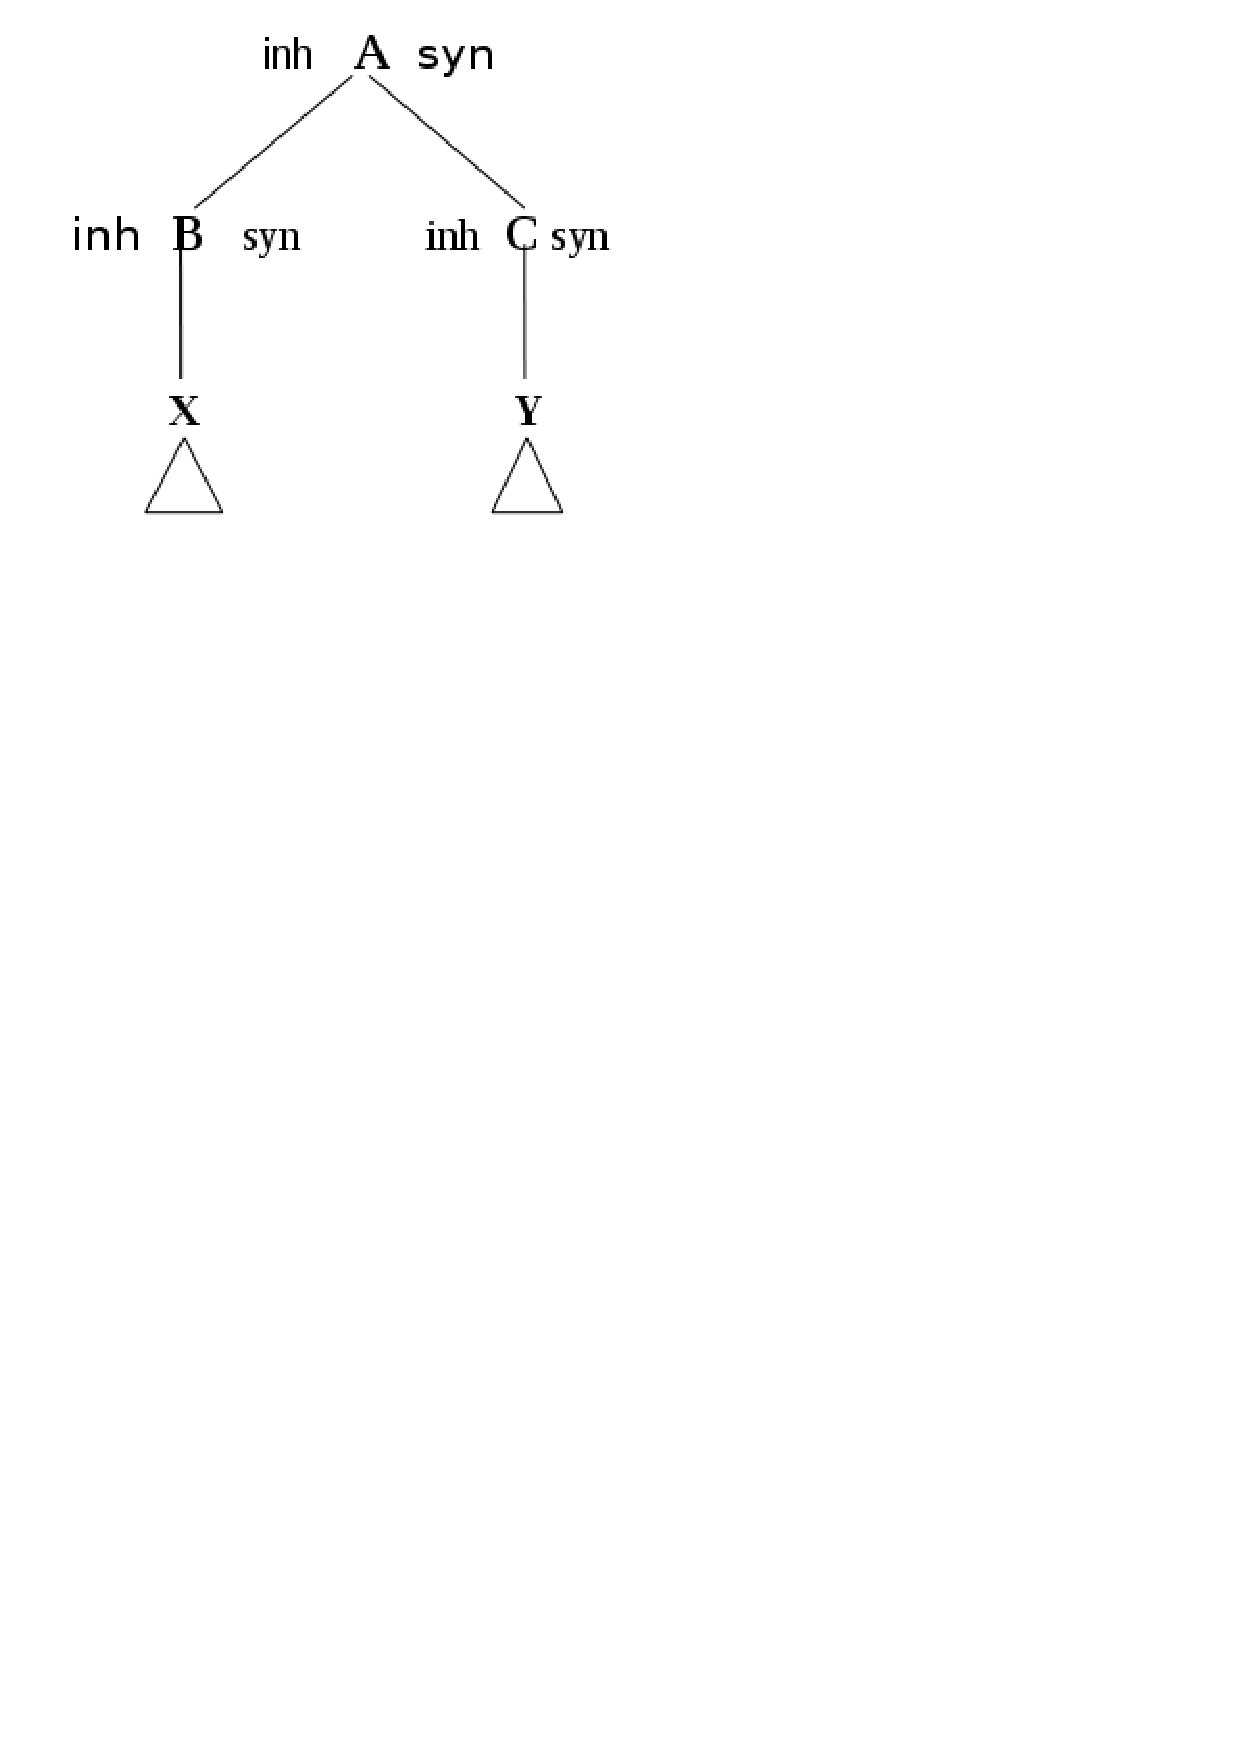
\includegraphics[scale=0.4]{q5}
\end{figure}
The attributes X.syn and Y.syn are calculated at the children of B and C respectively. X.syn can depend of X.inh and on values in the triangle below X; similarly for Y.syn.
\begin{enumerate}
\item A is invoked (viewing the traversal as a program) and is passed its inherited attributes (A.inh in our case, but of course there could be several such attributes), which have been evaluated at its parent.
\item B is invoked by A and is given B.inh, which A has calculated. In programming terms: A executes
\begin{itemize}
\item[ ] call B(B.inh)
\item[ ]  where the argument has been evaluated by A. This argument can depend on A.inh since the parent of A has given A this value.
\end{itemize}
\item B calls its first child (in our example X is the only child) and passes to the child the child's inherited attributes. In programming terms: B executes
\begin{itemize}
\item[ ] call X(X.inh)
\end{itemize}
\item The child returns, passing back to B the synthesized attributes of the child. In programming terms: X executes
\begin{itemize}
\item[ ] return X.syn
\item[ ] In reality there could be more synthesized attributes, there could be more children, the children could have children, etc.
\end{itemize}
\item B returns to A passing back B.syn, which can depend on B.inh (given to B by A in step 2) and X.syn (given to B by X in the previous step).
\item A calls C giving C its inherited attributes, which can depend on A.inh (given to A, by A's parent), B.inh (previously calculated by A in step 2), and B.syn (given to A by B in step 5).
\item C calls its first child, just as B did.
\item The child returns to C, just as B's child returned to B.
\item C returns to A passing back C.syn, just as B did.
\item A returns to its parent passing back A.syn, which can depend on A.inh (given to A by its parent in step 1), B.inh calculated by A in step 2, B.syn (given to A by B in step 5), C.inh (calculated by A in step 6), and C.syn (given to A by C in step 9).
\end{enumerate}

\noindent
Formally do a depth first traversal of the tree and evaluate inherited attributes on the way down and synthetic attributes on the way up. This corresponds to an Euler-tour traversal. It also corresponds to a call graph of a program where actions are taken at each call and each return.\\
6. Describe and differentiate between synthesized and inherited attributes.\\
\emph{Answer}:

\textbf{Synthesized attributes} are those attributes whose values are only in productions in which their symbol appears on the left-hand side.For annotated parse trees this means that the attribute flow --- the pattern in
which information moves from node to node is entirely bottom-up.    An attribute grammar in which all attributes are synthesized is said to be S-attributed. The arguments to semantic functions in an S-attributed grammar are always attributes of symbols on the right-hand side of the current production, and the return value is always placed into an attribute of the left-hand
side of the production.

Attributes whose values are calculated when their symbol is on the right-hand side of the current production are said to be \textbf{inherited attributes}. They allow contextual information to flow into a symbol from above or from the side, so that the rules of that production can be enforced in different ways (or generate different values) depending on surrounding context. Symbol table information is commonly passed from symbol to symbol by means of inherited attributes. Inherited attributes of the root of the parse tree can also be used to represent the external environment.\\
\\
\\
\\
\noindent
7. Show the stack with all activation record instances, including the dynamic chain, when
execution reaches position 1 in the following skeletal program. This program uses the deep-
access method to implement dynamic scoping.\\
void fun1() \{\\
float a;\\
...\\
\}\\
void fun2() \{\\
int b, c;\\
...\\
\}\\
void fun3() \{\\
float d;\\
... \verb+       + $\longleftarrow$ 1\\
\}\\
void main() \{\\
char e, f, g;\\
...\\
\}\\
The calling sequence for this program for execution to reach fun3 is:\\
main calls fun2\\
fun2 calls fun1\\
fun1 calls fun1\\
fun1 calls fun3\\
\emph{Answer}:\\
If local variables are stack dynamic and are part of the activation records in a
dynamic-scoped language, references to nonlocal variables can be resolved by
searching through the activation record instances of the other subprograms
that are currently active, beginning with the one most recently activated.

The dynamic chain links together all subprogram activation record instances in the reverse of the order in which they were activated. Therefore, the dynamic chain is exactly what is needed to reference
nonlocal variables in a dynamic-scoped language. This method is called deep
access, because access may require searches deep into the stack.

The activation records for the given code example is:\\
\begin{figure}
\centering
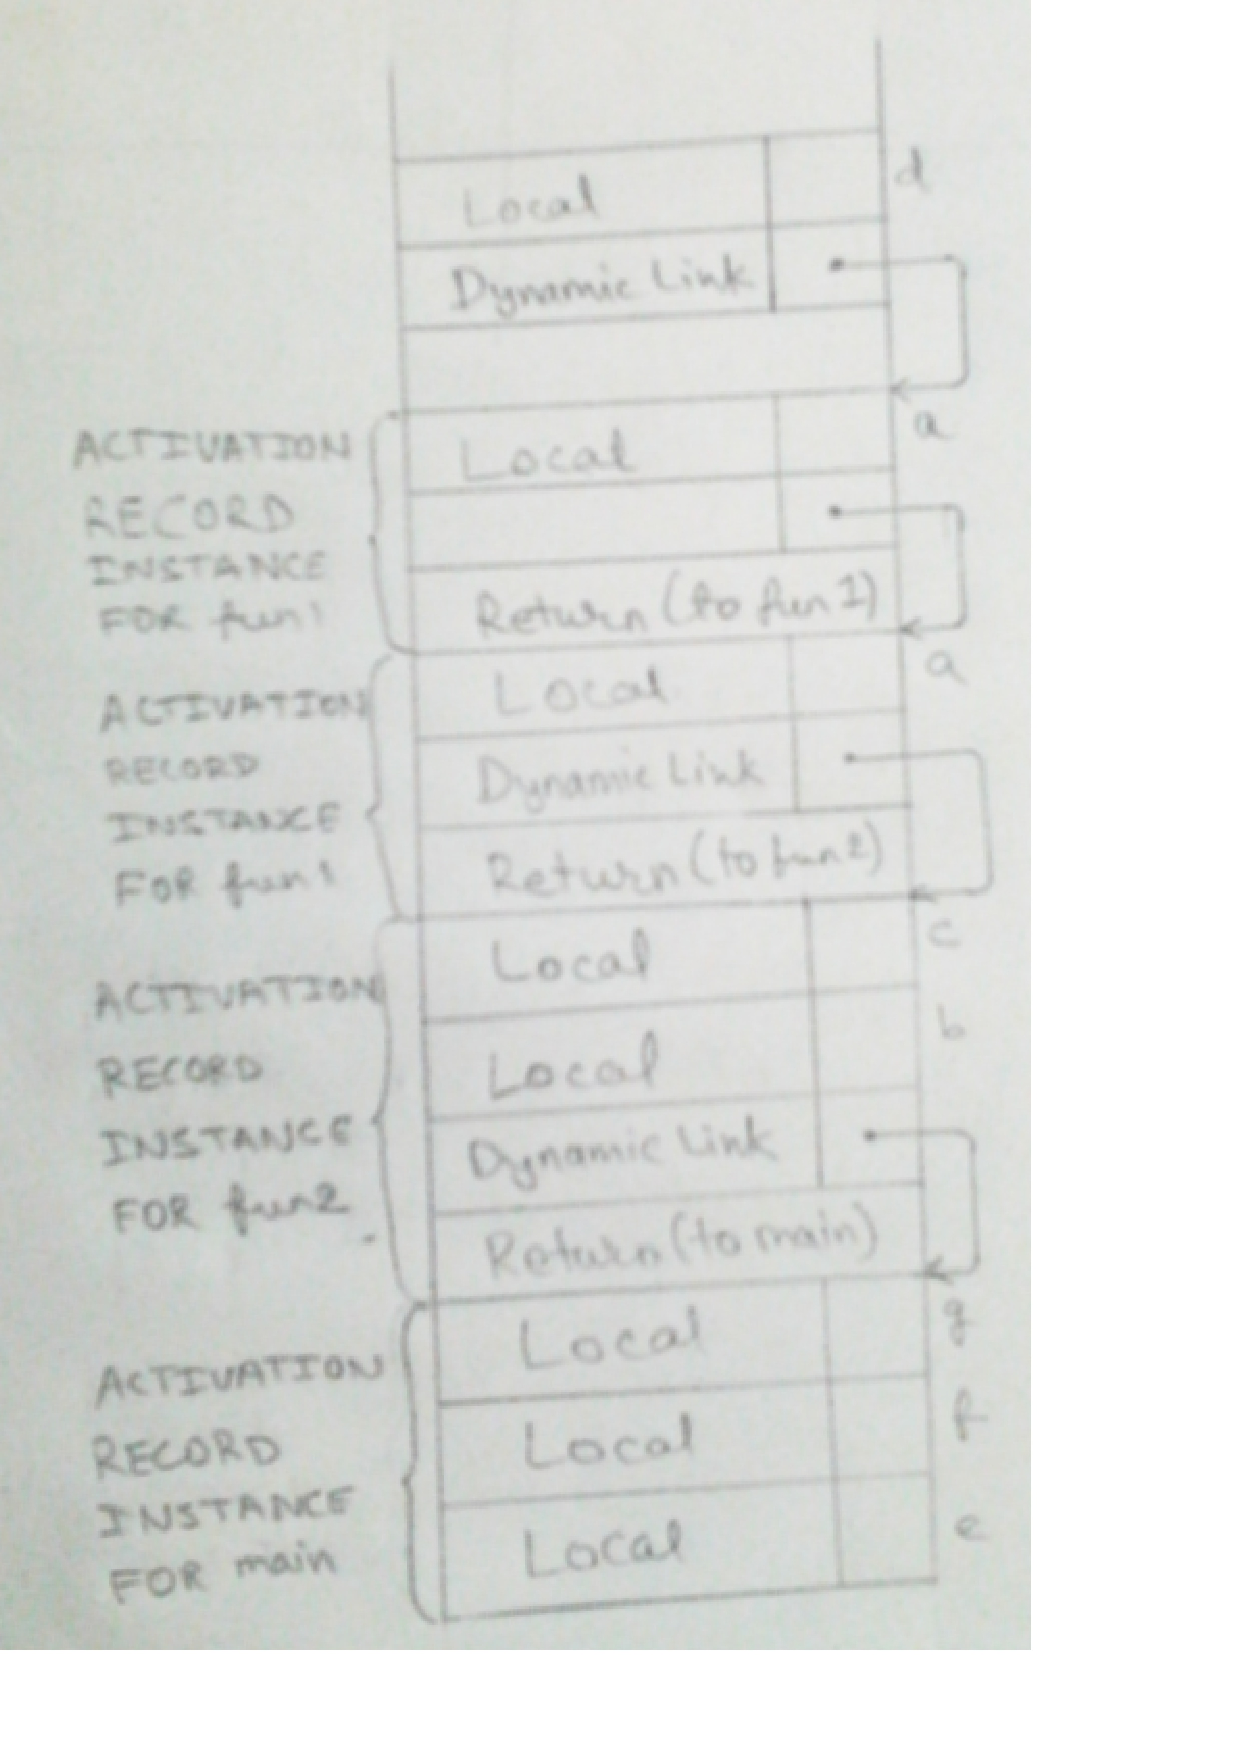
\includegraphics[scale=0.6]{q7}
\end{figure}
\pagebreak
\\
\\
\\
\\
\\
\\
\\
\noindent
8. Design a skeletal program and a calling sequence that results in an activation
   record instance in which the static and dynamic links point to different
   activation-recorded instances in the run-time stack. \\
\emph{Answer}:\\
procedure Main\_2 is\\
\verb+    + X : Integer;\\
\verb+    +procedure Bigsub is\\
\verb+    +\verb+    +    A, B, C : Integer;\\
\verb+    +\verb+    +    procedure Sub1 is\\
\verb+    +\verb+    +\verb+    +    A, D : Integer;\\
\verb+    +\verb+    +\verb+    +    begin -- of Sub1\\
\verb+    +\verb+    +\verb+    +    A := B + C; $\longleftarrow$ 1\\
\verb+    +\verb+    +\verb+    +      ...\\
\verb+    +    end; -- of Sub1\\
\verb+    +    procedure Sub2(X : Integer) is\\
\verb+    +\verb+    +      B, E : Integer;\\
\verb+    +\verb+    +      procedure Sub3 is\\
\verb+    +\verb+    +\verb+    +        C, E : Integer;\\
\verb+    +\verb+    +\verb+    +        begin -- of Sub3\\
\verb+    +\verb+    +\verb+    +        ...\\
\verb+    +\verb+    +\verb+    +        Sub1;\\
\verb+    +\verb+    +\verb+    +        ...\\
\verb+    +\verb+    +\verb+    +        E := B + A; $\longleftarrow$ 2\\
\verb+    +\verb+    +      end; -- of Sub3\\
\verb+    +\verb+    +      begin -- of Sub2\\
\verb+    +\verb+    +      ...\\
\verb+    +\verb+    +      Sub3;\\
\verb+    +\verb+    +      ...\\
\verb+    +\verb+    +      A := D + E; $\longleftarrow$ 3\\
\verb+    +    end; -- of Sub2\\
\verb+    +    begin -- of Bigsub\\
\verb+    +\verb+    +    ...\\
\verb+    +\verb+    +    Sub2(7);\\
\verb+    +\verb+    +    ...\\
\verb+    +  end; -- of Bigsub\\
  begin -- of Main\_2\\
\verb+    +  ...\\
\verb+    +  Bigsub;\\
\verb+    +  ...\\
end; -- of Main\_2\\
\\
The sequence of procedure calls is:\\
Main\_2 calls Bigsub\\
Bigsub calls Sub2\\
Sub2 calls Sub3\\
Sub3 calls Sub1\\
\\
The activation records with static and dynamic links is as follows:\\
\begin{figure}
\centering
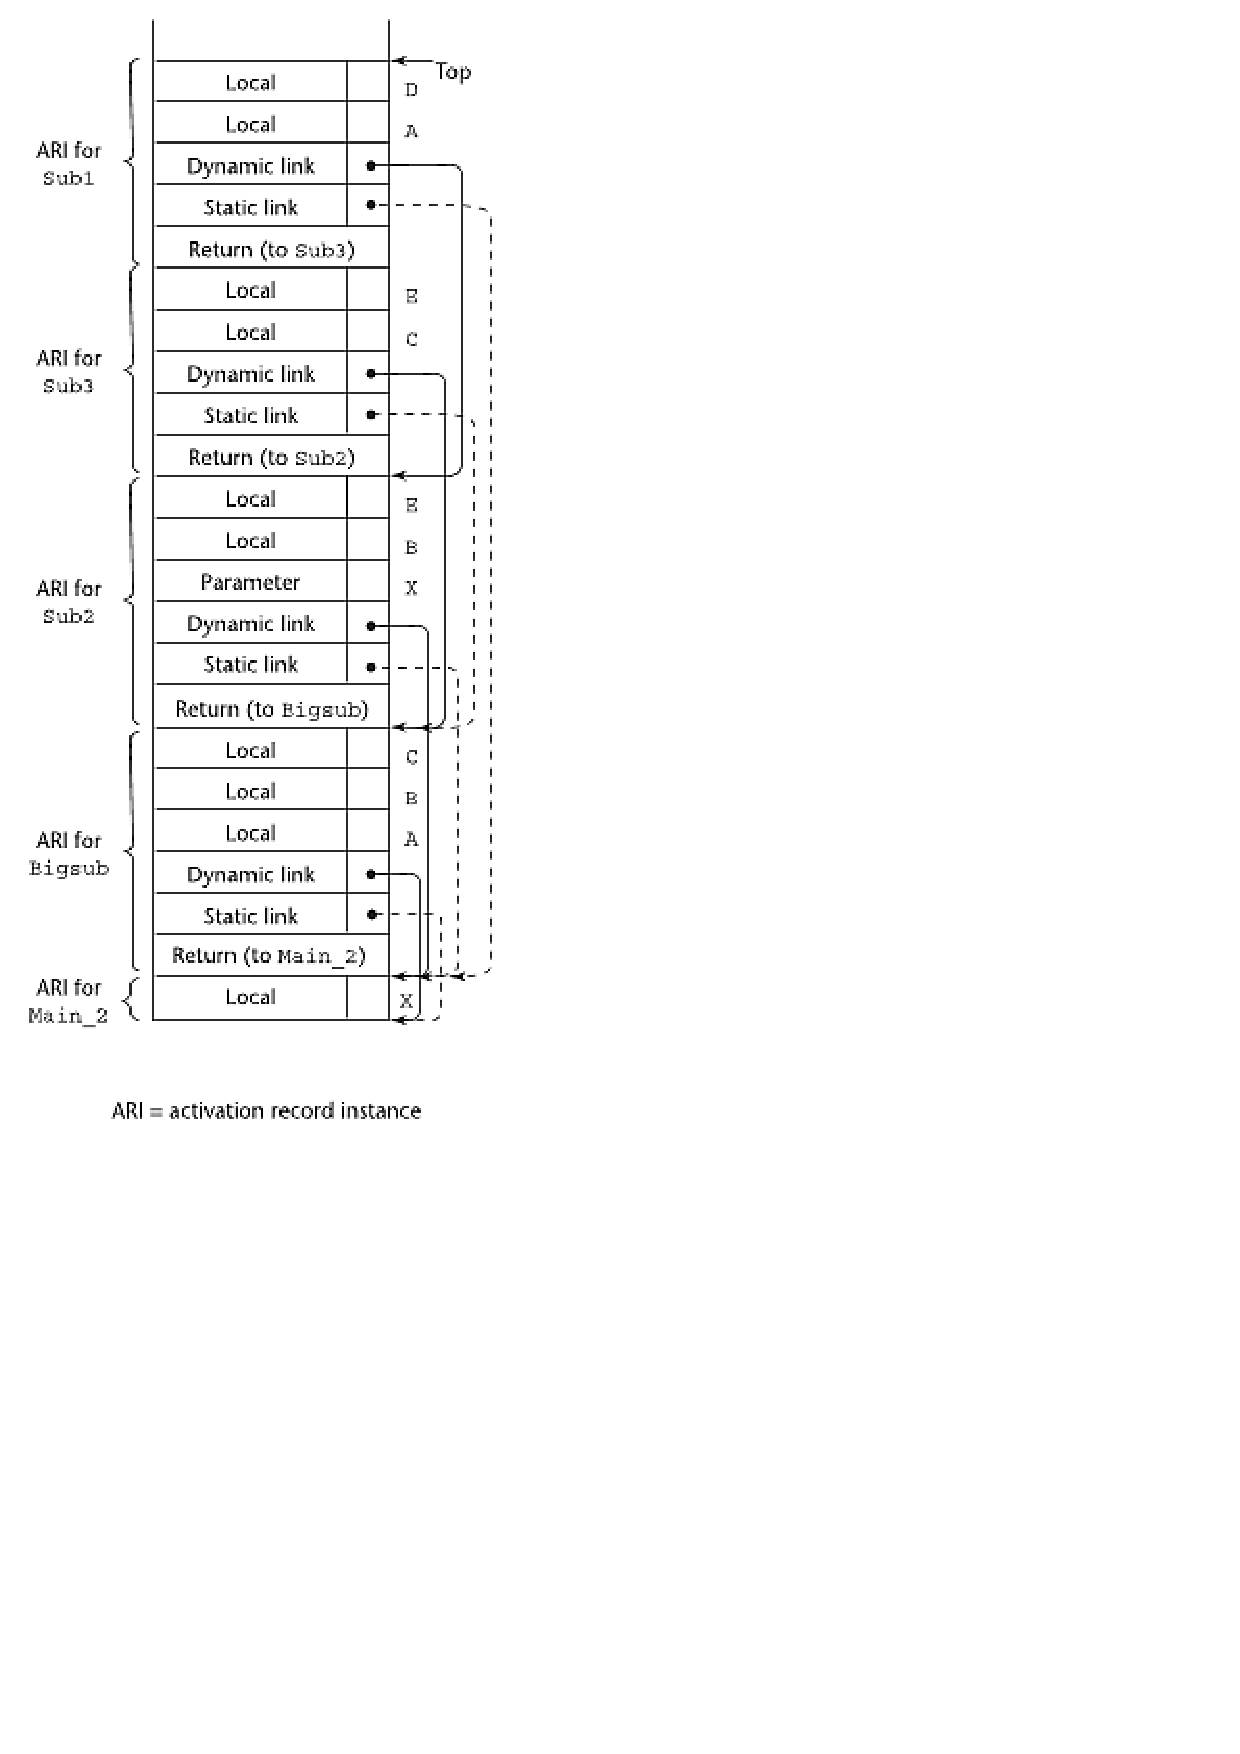
\includegraphics[scale=0.5]{ari}
\end{figure}

     At position 1 in procedure Sub1, the reference is to the local variable,
A, not to the nonlocal variable A from Bigsub. This reference to A has the
chain\_offset/local\_offset pair (0, 3). The reference to B is to the nonlocal B
from Bigsub. It can be represented by the pair (1, 4). The local\_offset is 4,
because a 3 offset would be the first local variable (Bigsub has no parameters). Notice that if the dynamic link were used to do a simple search for
an activation record instance with a declaration for the variable B, it would
find the variable B declared in Sub2, which would be incorrect. If the (1, 4)
pair were used with the dynamic chain, the variable E from Sub3 would be
used. The static link, however, points to the activation record for Bigsub,
which has the correct version of B . The variable B in Sub2 is not in the
referencing environment at this point and is (correctly) not accessible. The
reference to C at point 1 is to the C defined in Bigsub, which is represented
by the pair (1, 5).\\
\\
\noindent
9. What does it mean for an attribute grammar to be S-attributed? L-attributed? Noncircular? What is the significance of these grammar classes?
\\
\emph{Answer}:\\
   An attribute grammar in which all attributes are synthesized is said to be \textbf{S-attributed}. The arguments to semantic functions in an S-attributed grammar are always attributes of symbols on the right-hand side of the current production, and the return value is always placed into an attribute of the left-hand side of the production. Tokens (terminals) often have intrinsic properties (e.g.,
the character-string representation of an identifier or the value of a numeric constant); in a compiler these are synthesized attributes initialized by the scanner.

An \textbf{L-attributed} grammar is where attributes can be evaluated by visiting the nodes of the parse tree in a single left-to-right, depth-first traversal (the same order in which they are visited during a top-down parse). \\Formally, it follows the following rules:\\
\begin{itemize}
\item Each synthesized attribute of of a left-hand side symbol depends only on that symbol's inherited attributes or on attributes (synthesized or inherited) of the the production's right-hand side symbols; and
\item each inherited attribute of a right-hand side symbol depends only on inherited attributes of the left-hand side symbol or on attributes (synthesized or inherited) of symbols to its left on the right-hand side.
\end{itemize}

An attribute grammar is \textit{noncircular} if it never leads to a parse tree in which there are cycles in the attribute
flow graph --- that is, if no attribute, in any parse tree, ever depends (transitively) on itself.

\textbf{Significance}:    S-attributed grammars are the most general class of attribute grammars for which evaluation can be implemented on-the-fly during an LR parse. L-attributed grammars are a proper superset of S-attributed grammars. They are the most general class of attribute grammars for which evaluation can be implemented on-the-fly during an LL parse.\\
\\
\noindent
10. Explain Space Management Attributes for Context-free grammar for a calculator language.\\
\emph{Answer}:\\
Any attribute evaluation method requires space to hold the attributes of the
grammar symbols. If we are building an explicit parse tree, then the obvious approach is to store attributes in the nodes of the tree themselves. If we are not building a parse tree, then we need to find a way to keep track of the attributes
for the symbols we have seen (or predicted) but not yet finished parsing. The details differ in bottom-up and top-down parsers.

For a bottom-up parser with an S-attributed grammar:
\begin{itemize}
\item maintain an attribute stack that directly mirrors the parse stack
\begin{itemize}
\item next to every state number on the parse stack is an attribute record for the symbol we shifted when we entered that state.
\end {itemize}
\end {itemize}

The context-free grammar for a calculator language is:\\
\begin{quote}
1. $E_1$ $\longrightarrow$ $E_2$ + T \\
\verb+       +$\triangleright$ $E_1$.val := sum($E_2$.val + T.val)\\
2. $E_1$ $\longrightarrow$ $E_2$ - T \\
\verb+       +$\triangleright$ $E_1$.val := sum($E_2$.val - T.val)\\
3. E $\longrightarrow$  T \\
\verb+       +$\triangleright$ E.val := T.val\\
4. $T_1$ $\longrightarrow$ $T_2$ * F \\
\verb+       +$\triangleright$ $T_1$.val := product($T_2$.val * F.val)\\
5. $T_1$ $\longrightarrow$ $T_2$ / F \\
\verb+       +$\triangleright$ $T_1$.val := quotient($T_2$.val / F.val)\\
6. T $\longrightarrow$  F \\
\verb+       +$\triangleright$ T.val := F.val\\
7. $F_1$ $\longrightarrow$ $-F_2$\\
\verb+       +$\triangleright$ $F_1$.val := additive\_inverse($F_2$.val)\\
8. F $\longrightarrow$  (E) \\
\verb+       +$\triangleright$ F.val := E.val\\
9. F $\longrightarrow$ const\\
\verb+       +$\triangleright$ F.val := const\\
\end{quote}
We can use the approach described above for bottom-up parser and all the attributes in this grammar are synthesized.
For example, consider the parse tree below for the expression (1+3) * 2. The val attributes of symbols are shown in boxes. Curved arrows represent the attribute flow, which is strictly upward in this case.
\begin{figure}[!hbp]
\centering
\includegraphics[scale=0.45]{agq10}
\caption{Decoration of a parse tree for (1 + 3) * 2 }
\end{figure}
\end{document}
